\documentclass[11pt]{article}
\usepackage[textwidth=18.0cm, textheight=23.0cm, top=2.0cm]{geometry}
\usepackage{pst-all}
\usepackage{amssymb}
\usepackage{tikz}
\usepackage{underscore}\begin{document}
\pagestyle{empty}


ClassName: \underline{\textbf{Class_07.2bp-6}}
\par
BinSize: \underline{\textbf{100 × 100}}
\par
ReduceSize: \underline{\textbf{100 × 100}}
\par
TypeNum: \underline{\textbf{20}}
\par
Num: \underline{\textbf{20}}
\par
OutS: \underline{\textbf{40000}}
\par
InS: \underline{\textbf{32742}}
\par
Rate: \underline{\textbf{0.819}}
\par
UB: \underline{\textbf{4}}
\par
LB0: \underline{\textbf{4}}
\par
LB: \underline{\textbf{4}}
\par
LBWithCut: \underline{\textbf{4}}
\par
NodeCut: \underline{\textbf{0}}
\par
ExtendedNodeCnt: \underline{\textbf{1}}
\par
GenNodeCnt: \underline{\textbf{1}}
\par
PrimalNode: \underline{\textbf{0}}
\par
ColumnCount: \underline{\textbf{4}}
\par
TotalCutCount: \underline{\textbf{0}}
\par
RootCutCount: \underline{\textbf{0}}
\par
LPSolverCnt: \underline{\textbf{1}}
\par
PricingSolverCnt: \underline{\textbf{0}}
\par
BranchAndBoundNum: \underline{\textbf{1}}
\par
isOpt: \underline{\textbf{true}}
\par
TimeOnInitSolution: \underline{\textbf{0.000 s}}
\par
TimeOnPrimal: \underline{\textbf{0.000 s}}
\par
TimeOnPricing: \underline{\textbf{0.000 s}}
\par
TimeOnRmp: \underline{\textbf{0.078 s}}
\par
TotalTime: \underline{\textbf{0.125 s}}
\par
\newpage


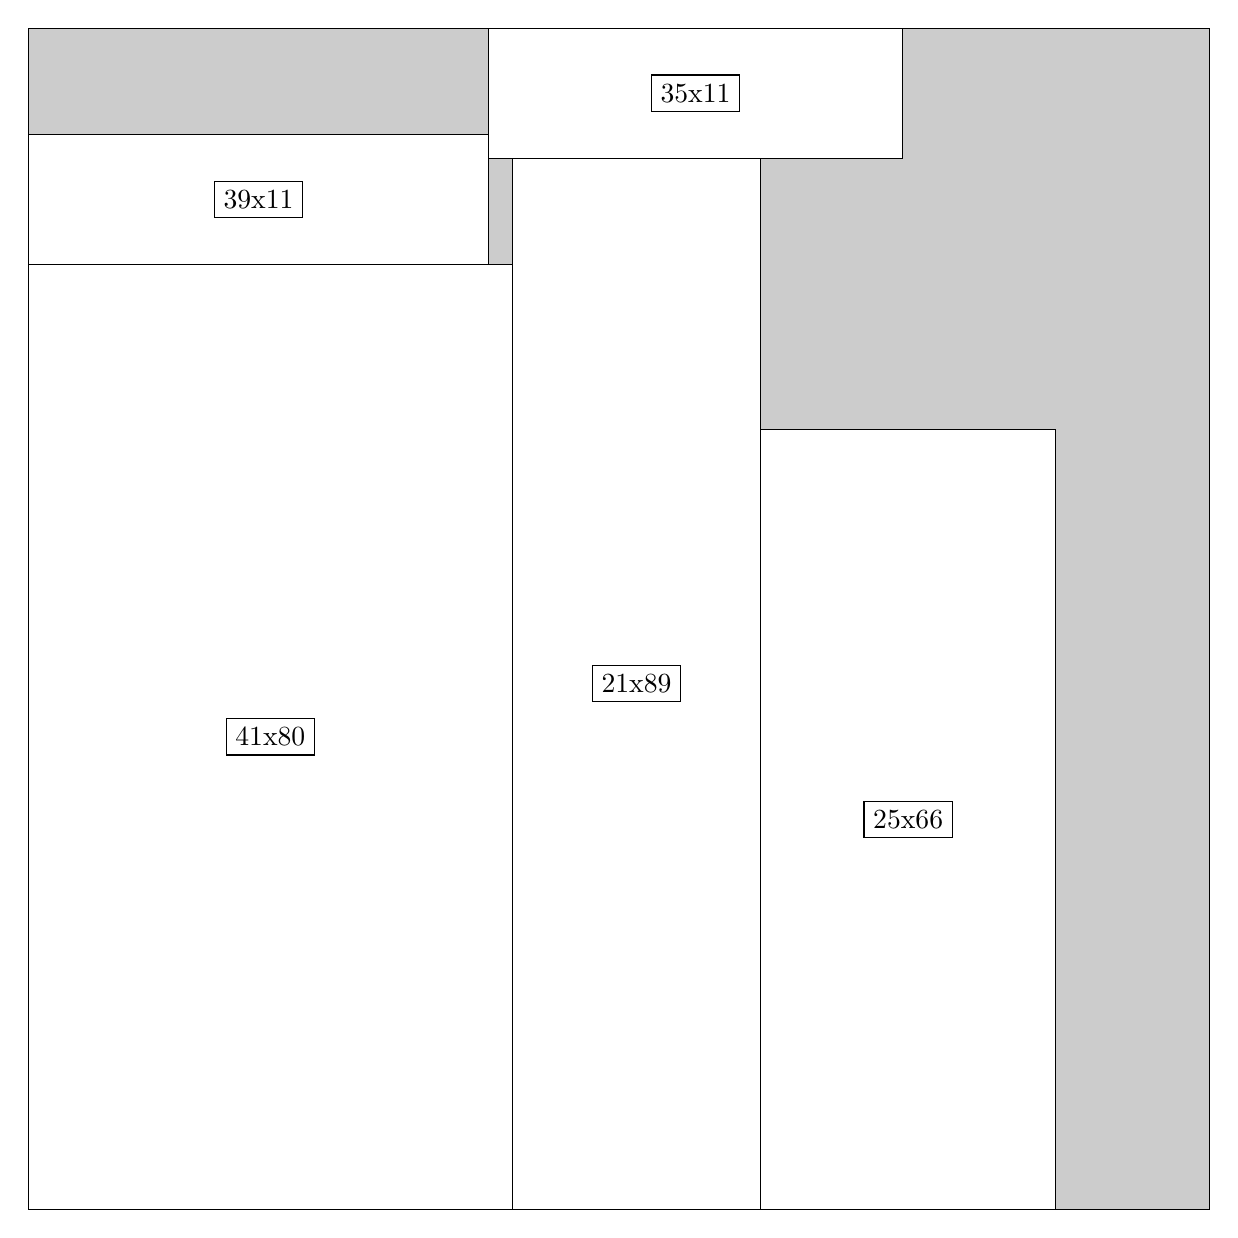
\begin{tikzpicture}[shorten >=1pt,scale=1.0,every node/.style={scale=1.0},->]
\tikzstyle{vertex}=[circle,fill=black!25,minimum size=14pt,inner sep=0pt]
\filldraw[fill=gray!40!white, draw=black] (0,0) rectangle (15.0,15.0);
\foreach \name/\x/\y/\w/\h in {41x80/0.0/0.0/6.1499999999999995/12.0,25x66/9.299999999999999/0.0/3.75/9.9,21x89/6.1499999999999995/0.0/3.15/13.35,39x11/0.0/12.0/5.85/1.65,35x11/5.85/13.35/5.25/1.65}
\filldraw[fill=white!40!white, draw=black] (\x,\y) rectangle node[draw] (\name) {\name} ++(\w,\h);
\end{tikzpicture}


w =41 , h =80 , x =0 , y =0 , v =3280
\par
w =25 , h =66 , x =62 , y =0 , v =1650
\par
w =21 , h =89 , x =41 , y =0 , v =1869
\par
w =39 , h =11 , x =0 , y =80 , v =429
\par
w =35 , h =11 , x =39 , y =89 , v =385
\par
\newpage


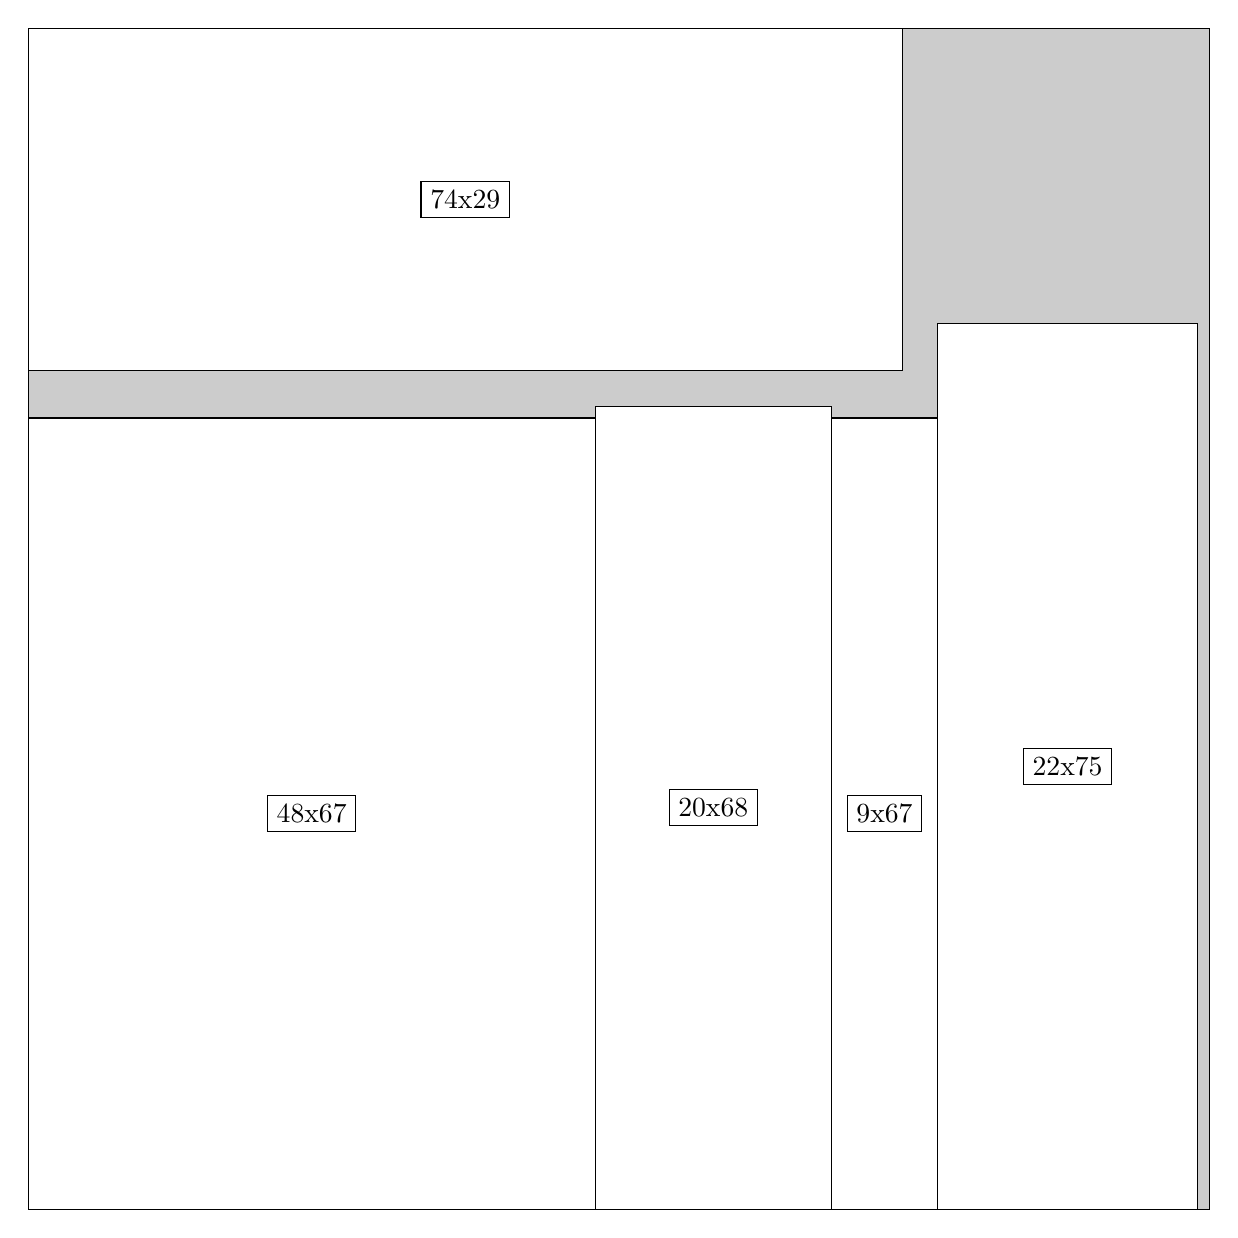
\begin{tikzpicture}[shorten >=1pt,scale=1.0,every node/.style={scale=1.0},->]
\tikzstyle{vertex}=[circle,fill=black!25,minimum size=14pt,inner sep=0pt]
\filldraw[fill=gray!40!white, draw=black] (0,0) rectangle (15.0,15.0);
\foreach \name/\x/\y/\w/\h in {48x67/0.0/0.0/7.199999999999999/10.049999999999999,74x29/0.0/10.65/11.1/4.35,20x68/7.199999999999999/0.0/3.0/10.2,22x75/11.549999999999999/0.0/3.3/11.25,9x67/10.2/0.0/1.3499999999999999/10.049999999999999}
\filldraw[fill=white!40!white, draw=black] (\x,\y) rectangle node[draw] (\name) {\name} ++(\w,\h);
\end{tikzpicture}


w =48 , h =67 , x =0 , y =0 , v =3216
\par
w =74 , h =29 , x =0 , y =71 , v =2146
\par
w =20 , h =68 , x =48 , y =0 , v =1360
\par
w =22 , h =75 , x =77 , y =0 , v =1650
\par
w =9 , h =67 , x =68 , y =0 , v =603
\par
\newpage


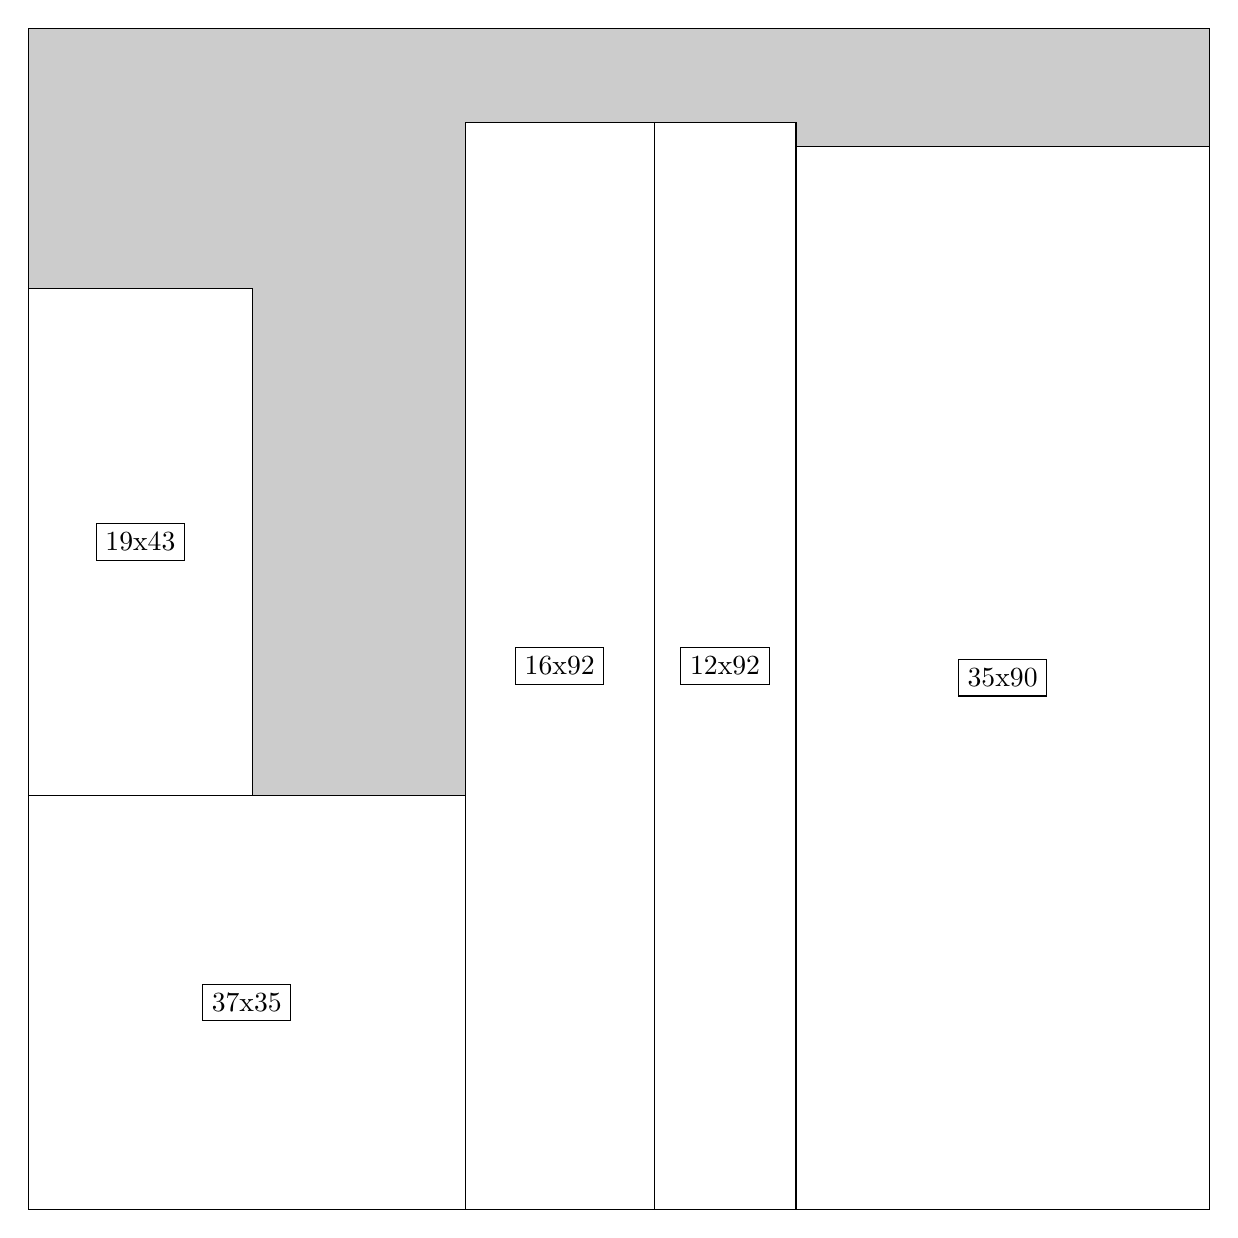
\begin{tikzpicture}[shorten >=1pt,scale=1.0,every node/.style={scale=1.0},->]
\tikzstyle{vertex}=[circle,fill=black!25,minimum size=14pt,inner sep=0pt]
\filldraw[fill=gray!40!white, draw=black] (0,0) rectangle (15.0,15.0);
\foreach \name/\x/\y/\w/\h in {35x90/9.75/0.0/5.25/13.5,16x92/5.55/0.0/2.4/13.799999999999999,37x35/0.0/0.0/5.55/5.25,12x92/7.949999999999999/0.0/1.7999999999999998/13.799999999999999,19x43/0.0/5.25/2.85/6.45}
\filldraw[fill=white!40!white, draw=black] (\x,\y) rectangle node[draw] (\name) {\name} ++(\w,\h);
\end{tikzpicture}


w =35 , h =90 , x =65 , y =0 , v =3150
\par
w =16 , h =92 , x =37 , y =0 , v =1472
\par
w =37 , h =35 , x =0 , y =0 , v =1295
\par
w =12 , h =92 , x =53 , y =0 , v =1104
\par
w =19 , h =43 , x =0 , y =35 , v =817
\par
\newpage


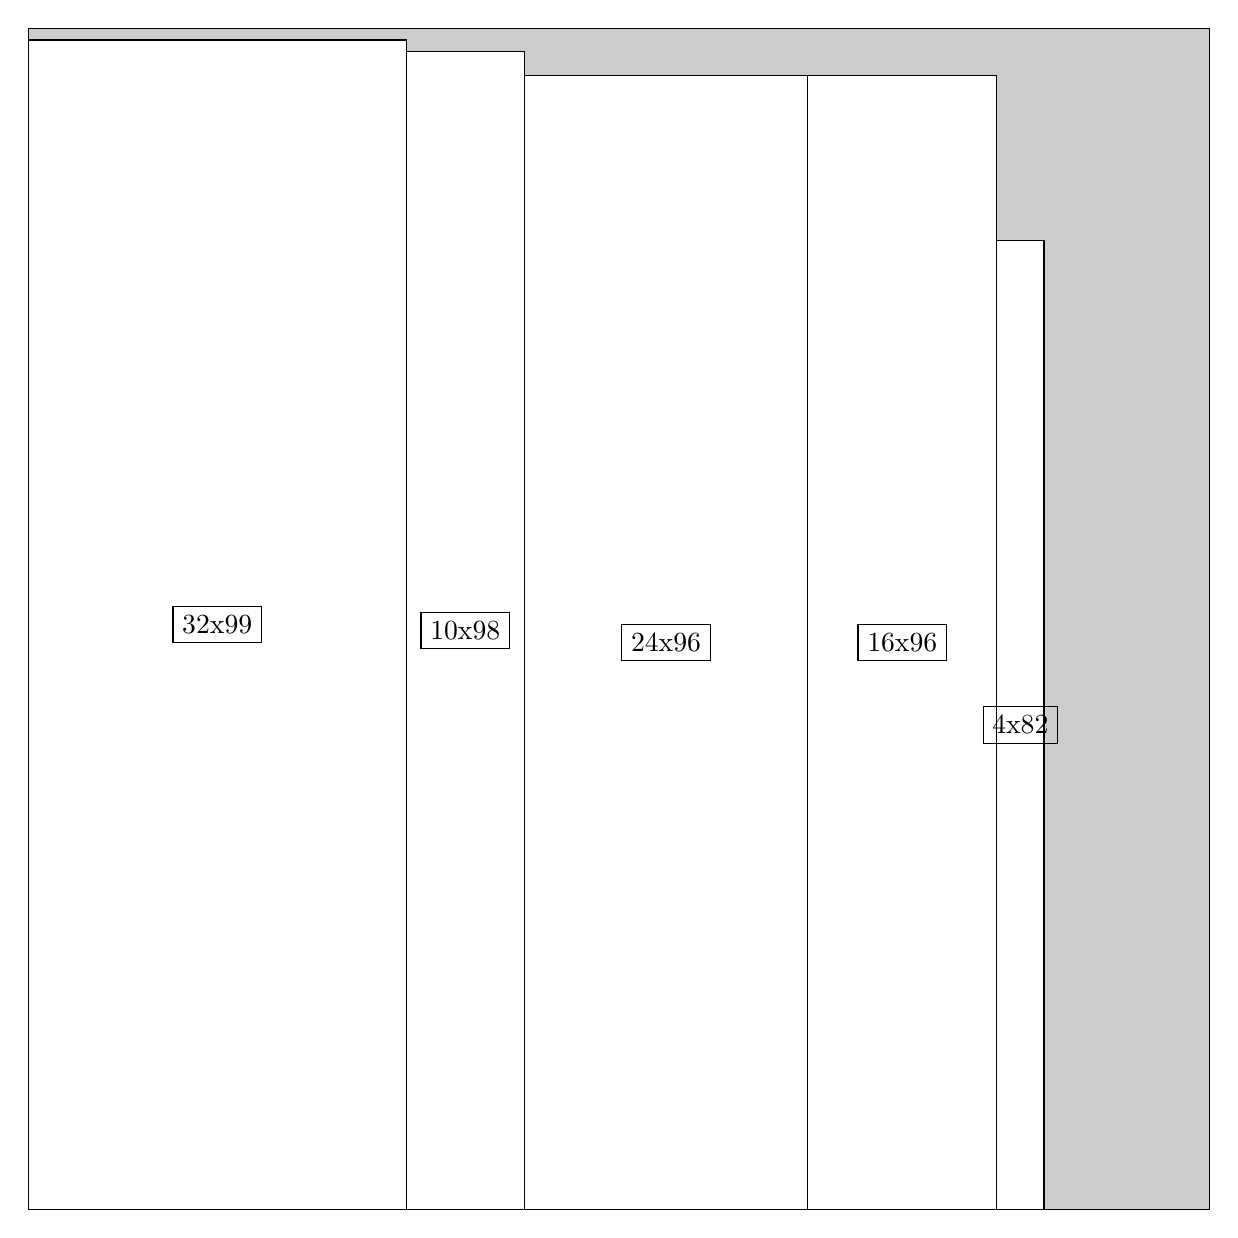
\begin{tikzpicture}[shorten >=1pt,scale=1.0,every node/.style={scale=1.0},->]
\tikzstyle{vertex}=[circle,fill=black!25,minimum size=14pt,inner sep=0pt]
\filldraw[fill=gray!40!white, draw=black] (0,0) rectangle (15.0,15.0);
\foreach \name/\x/\y/\w/\h in {32x99/0.0/0.0/4.8/14.85,24x96/6.3/0.0/3.5999999999999996/14.399999999999999,16x96/9.9/0.0/2.4/14.399999999999999,10x98/4.8/0.0/1.5/14.7,4x82/12.299999999999999/0.0/0.6/12.299999999999999}
\filldraw[fill=white!40!white, draw=black] (\x,\y) rectangle node[draw] (\name) {\name} ++(\w,\h);
\end{tikzpicture}


w =32 , h =99 , x =0 , y =0 , v =3168
\par
w =24 , h =96 , x =42 , y =0 , v =2304
\par
w =16 , h =96 , x =66 , y =0 , v =1536
\par
w =10 , h =98 , x =32 , y =0 , v =980
\par
w =4 , h =82 , x =82 , y =0 , v =328
\par
\newpage


\end{document}